\documentclass[journal, a4paper]{IEEEtran}


\usepackage[hidelinks]{hyperref}  % PDF Hyperlinks

\usepackage{enumitem}             % Lists
\usepackage{hanging}              % indent

\usepackage{lipsum}               % Lorem Ipsum


\usepackage{siunitx}              % SI Units
\usepackage{booktabs}             % Tables
\usepackage{multirow}
\usepackage{caption}              % Captions


\usepackage{graphicx}             % Images or Graphics
\usepackage{pgfplots}             % Graphs and Plots

% === Change subsection from A B C to 1.1 1.2 1.3 ===
\usepackage{alphalph}
\renewcommand\thesubsectiondis{\AlphAlph{\value{subsection}}.}
\renewcommand\thesubsection{\mbox{\thesection-\AlphAlph{\value{subsection}}}}
% ====================================================


\def\checkmark{\tikz\fill[scale=0.4](0,.35) -- (.25,0) -- (1,.7) -- (.25,.15) -- cycle;} 

\usetikzlibrary{mindmap}
\usetikzlibrary{positioning}
\usetikzlibrary{shapes,arrows}
\usetikzlibrary{shapes.geometric, arrows}

\tikzset{
    objRectangle/.style={rectangle, minimum width=3cm, minimum height=1cm, text centered, draw=black, text width = 5cm},
    objRoundRectangle/.style={rectangle, rounded corners, minimum width=3cm, minimum height=1cm, text centered, draw=black, text width = 5cm},
    objRectangleMethods/.style={rectangle, minimum height=1cm, text centered, draw=black, text width = 3cm},
    arrow/.style={thick, ->, >=stealth}
}

% correct bad hyphenation here
\hyphenation{op-tical net-works semi-conduc-tor}


\begin{document}
\title{A Literature Review on Non-Destructive Testing and Structural Health Monitoring}


% === Authors === %
\author{Antonette~C.~Maxey,~\IEEEmembership{CPE Student,~MMCM,}
        Florencio~N.~Pulido,~\IEEEmembership{CPE Student,~MMCM,}
        and~Vincent~Alfred~B.~Tomas,~\IEEEmembership{ECE Student,~MMCM}% <-this % stops a space
}



% The paper headers
\markboth{Methods of Research Literature Review, February~2024 65d819b0}%
{Shell \MakeLowercase{\textit{et al.}}: Developing a Portable NDT Device for Efficient SHM}


% === Build Title Area  === %
\maketitle


\begin{abstract}
  This literature review focuses on the advancements and challenges in Structural Health Monitoring (SHM)
  through the lens of portable Non-Destructive Testing (NDT) devices.
  These devices offer promising solutions to the limitations of traditional SHM methods, such as high cost and complexity.
  This review encompasses various aspects including existing portable NDT devices, sensor technology,
  data acquisition and analysis, as well as applications and case studies. It identifies significant advancements
  in sensor technologies and data analytics for NDT and SHM, while also highlighting critical limitations and research gaps.
  The synthesis and critique section emphasize the need for improvements in sensor accuracy, data processing capabilities,
  and environmental robustness for optimal infrastructure safety. Future developments in portable NDT devices are seen
  in the integration of advanced technologies like embedded systems, wireless sensors, cloud computing, and artificial intelligence.
  The findings underscore the importance of addressing these challenges for the successful deployment of portable NDT
  devices in SHM applications, paving the way for enhanced efficiency and accessibility in ensuring structural integrity.
\end{abstract}


% Note that keywords are not normally used for peerreview papers.
\begin{IEEEkeywords}
  NDT, SHM, damage.
\end{IEEEkeywords}







\section{Introduction}
\IEEEPARstart{S}{tructural} Health Monitoring (SHM) is a pivotal engineering tool, providing real-time structural integrity data,
thereby ensuring safety and averting infrastructure failures \cite{gharehbaghi_critical_2022} \cite{katam_review_2023}.
Traditional SHM methods, while effective, are often limited by factors such as
high cost, complexity, and accessibility issues \cite{katam_review_2023} \cite{gharehbaghi_critical_2022}.
A portable, Non-Destructive Testing (NDT) device presents a promising solution for efficient and accessible SHM,
overcoming the limitations of traditional methods \cite{guo_portable_2022} \cite{chen_research_2023}.
The objective of this capstone project is to explore the potential of a portable,
NDT device in overcoming the limitations of traditional SHM methods.

SHM is a field dedicated to the ongoing monitoring and evaluation of the structural integrity
of various infrastructure systems \cite{katam_review_2023}, NDT is a method that enables the assessment
of structural degradation without causing actual damage to the structure itself \cite{katam_review_2023},
and a portable NDT device is a tool that enhances the efficiency and accessibility of SHM \cite{hassani_systematic_2023} \cite{katam_review_2023}.
Various NDT methods, each with its unique advantages and disadvantages,
offer diverse approaches to assessing structural integrity without causing damage \cite{khedmatgozar_dolati_non-destructive_2021}.
Existing portable NDT devices, while offering promising functionalities,
also present certain limitations that need to be addressed for optimal SHM \cite{hassani_systematic_2023}.
Relevant theories and frameworks related to structural safety, damage detection,
and sensor technology play a crucial role in enhancing the effectiveness of SHM
and ensuring the safety of various infrastructures \cite{chen_sensor_2021} \cite{gharehbaghi_critical_2022}.


\section{Methodology}
This study employed both scientometric review and systematic review methodologies to identify the research gap in
Developing a Portable NDT Device for Efficient Structural Health Monitoring (SHM) construction.
The schematic representation of our methodology is illustrated in \autoref{fig:flowchartMethod}.


\begin{figure*}[ht]
  \centering
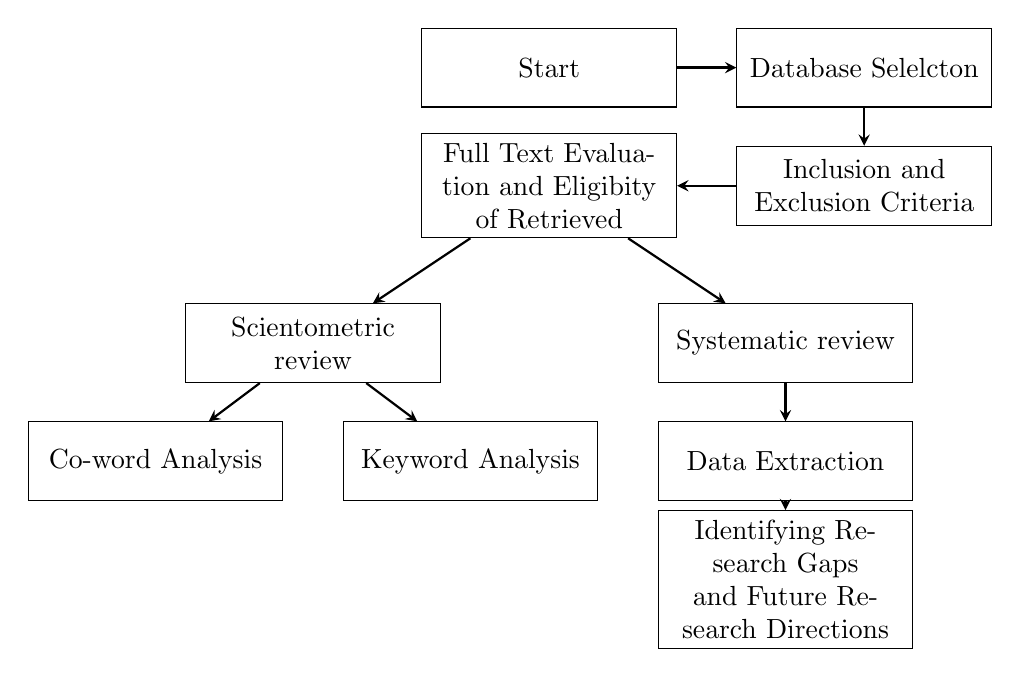
\begin{tikzpicture}[node distance=1.5cm]
  \node (001) [objRectangleMethods] {Start};
  \node (002) [objRectangleMethods, right of =001, xshift=2.5cm] {Database Selelcton};
  \node (003) [objRectangleMethods, below of=002] {Inclusion and Exclusion Criteria};
  \node (004) [objRectangleMethods, left of =003, xshift=-2.5cm] {Full Text Evaluation and Eligibity of Retrieved};

  \node (sci0) [objRectangleMethods, below of=004, xshift=-3cm, yshift=-0.5cm] {Scientometric review};
  \node (sci1a) [objRectangleMethods, below of=sci0, xshift=-2cm] {Co-word Analysis};
  \node (sci1b) [objRectangleMethods, below of=sci0, xshift=2cm] {Keyword Analysis};


  \node (sys0) [objRectangleMethods, below of=004, xshift=3cm, yshift=-0.5cm] {Systematic review};
  \node (sys1) [objRectangleMethods, below of=sys0] {Data Extraction};
  \node (sys2) [objRectangleMethods, below of=sys1] {Identifying Research Gaps and Future Research Directions};
  
  \draw[arrow] (001) -- (002);
  \draw[arrow] (002) -- (003);
  \draw[arrow] (003) -- (004);

  \draw[arrow] (004) -- (sci0);
  \draw[arrow] (sci0) -- (sci1a);
  \draw[arrow] (sci0) -- (sci1b);

  \draw[arrow] (004) -- (sys0);
  \draw[arrow] (sys0) -- (sys1);
  \draw[arrow] (sys1) -- (sys2);
\end{tikzpicture}
\caption{Outline of the Review Methodology}
\label{fig:flowchartMethod}
\end{figure*}


\subsection{Extraction and Evaluation of Research Data}
For our research, bibliometric data were extracted from \href{https://www.sciencedirect.com/}{ScienceDirect (Elsevier)} platform,
renowned for its extensive coverage of scientific publications especially those that correlate with the field of our study.

To proceed, two sets of keywords specifically Non-Destructive Testing and Structural Health Monitoring were carefully selected
to narrow down the search and only yield articles directly relevant to our study. 
The search yielded a substantial pool of one thousand one hundred sixty-nine (1,169) article titles.
However, to ensure the precision and relevance of our findings, we employed a meticulous process of refinement through the
application of exclusion and inclusion criteria.

First, we stragetically limited the publication timeframe from the years 2019 to 2023.
This allowed us to capture recent advancements and developments in our field of inquiry,
providing access to the most up-to-date research findings and methodologies.
The exclusion of the year 2024 was necessary as it had only just commenced, ensuring a focus on established research outcomes.

Secondly, we only considered articles falling within the subject area of engineering to ensure alignment with the
interdisciplinary nature of our research topic. By focusing on engineering-related publications, we aimed to draw
from a diverse range of studies and methodologies that contribute to the advancement of structural safety and non-destructive
testing techniques.

Furthermore, we adopted a selective approach in considering publications for inclusion, prioritizing research articles over
other forms of literature. The prioritization of articles from reputable engineering publications, such as Construction and
Building Materials, NDT \& E International, Structures, and Ultrasonics, was based on their relevance to our study aims and
their significance in the area.

Subsequent application of the inclusion and exclusion criteria resulted in the exclusion of
five hundred eighty-seven (587) articles based on year published, titles, and abstract screening.
Manual research gap analysis and text evaluation further refined the selection, leading to the exclusion of an
additional two hundred twenty-three (228) articles.
Among the remaining articles, one hundred sixty-five (165) underwent full-text evaluation,
and one hundred thirty-five (135) were excluded based on subject relevance and alignment with study objectives.

The application of our  methodological approach resulted in the inclusion of
thirty (30) studies that met the predefined criteria and were deemed suitable for further analysis and synthesis in our
research on developing a portable NDT device for efficient structural health monitoring as shown in \autoref{fig:flowchartFilter}.


\begin{figure}[hbtp]
  
    \centering
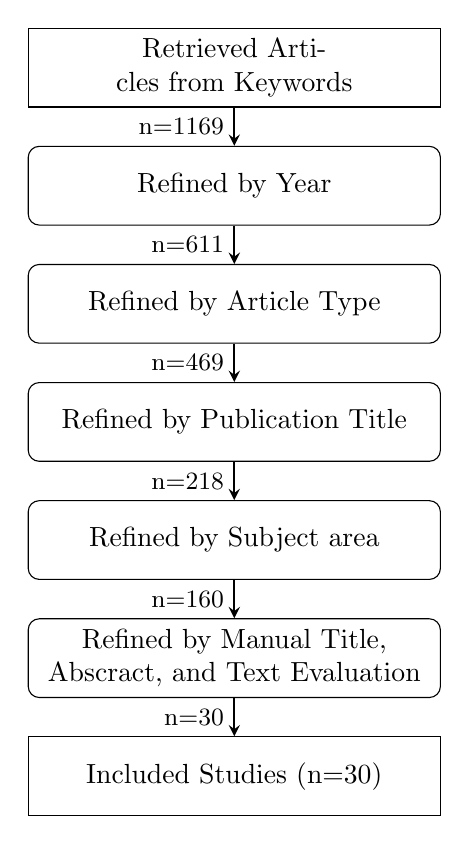
\begin{tikzpicture}[node distance=1.5cm]
    
    \node (001) [objRectangle] {Retrieved Articles from Keywords};
    \node (002) [objRoundRectangle, below of=001] {Refined by Year};
    \node (003) [objRoundRectangle, below of=002] {Refined by Article Type};
    \node (004) [objRoundRectangle, below of=003] {Refined by Publication Title};
    \node (005) [objRoundRectangle, below of=004] {Refined by Subject area};
    \node (006) [objRoundRectangle, below of=005] {Refined by Manual Title, Abscract, and Text Evaluation};
    \node (007) [objRectangle, below of=006] {Included Studies (n=30)};
    
    \draw [arrow] (001) -- node[anchor=east]{\small{n=1169}} (002);
    \draw [arrow] (002) -- node[anchor=east]{\small{n=611}} (003);
    \draw [arrow] (003) -- node[anchor=east]{\small{n=469}} (004);
    \draw [arrow] (004) -- node[anchor=east]{\small{n=218}} (005);
    \draw [arrow] (005) -- node[anchor=east]{\small{n=160}} (006);
    \draw [arrow] (006) -- node[anchor=east]{\small{n=30}} (007);

\end{tikzpicture}
\caption{Flowchart of the study selection process}
\label{fig:flowchartFilter}
\end{figure}





% === Results and Discussion of Scientometric Review === %
\section{Results and Discussion of Scientometric Review}
The thirty (30) articles were retrieved for this to conducted scientometric review.
\autoref{fig:publications} illustrates a distribution across publication years, with a notable increase in publications
from 2021 to 2023.
This trend suggests a growing interest and emphasis on advanced monitoring techniques,
aligning with the expanding need for structural integrity and safety assurance.
The concentration of publications in recent years reflects ongoing technological advancements,
particularly in sensor technology and data analytics.
Our study is positioned within this dynamic research landscape, aiming to leverage insights from existing
literature to inform and advance our research objectives.


\begin{figure}[hbtp]
  \centering

  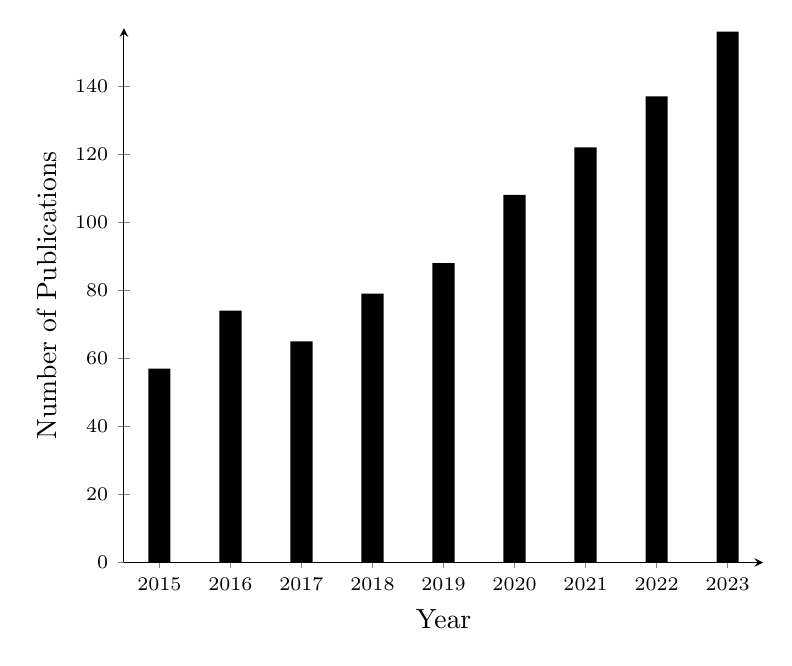
\begin{tikzpicture}
    \begin{axis}[
        ybar,
        width=0.8\columnwidth,                                          % Adjust the width of the plot
        bar width=8pt,                                                  % Adjust the width of the bars
        xlabel={Year},                                                  % Label for the x-axis
        ylabel={Number of Publications},                                % Label for the y-axis
        xtick=data,                                                     % Use data points as x-axis labels
        xticklabels={2015, 2016, 2017, 2018, 2019, 2020, 2021, 2022, 2023},                           % Labels for the x-axis ticks
        ticklabel style={font=\scriptsize}, % Set the font size for the x-axis tick labels
        ymin=0,                                                         % Set the minimum value for the y-axis
        enlarge y limits=0.1,                                           % Add space to the top and bottom of the y-axis
        legend style={draw=none}, % Remove the legend
        axis x line=bottom,  % Align x-axis line with ticks
        axis y line=left,    % Align y-axis line with ticks
        xmin=2014.5,                                                    % Set xmin to create a margin to the left of 2015
        xmax=2023.5,
        ymax=157,
    ]                                                 
      \addplot+ [fill=black, draw=none]  coordinates {(2015, 57) (2016, 74) (2017, 65)  (2018, 79) (2019, 88) (2020, 108) (2021, 122)  (2022, 137)  (2023, 156)};
    \end{axis}
  \end{tikzpicture}
  
  (\textit{a})

  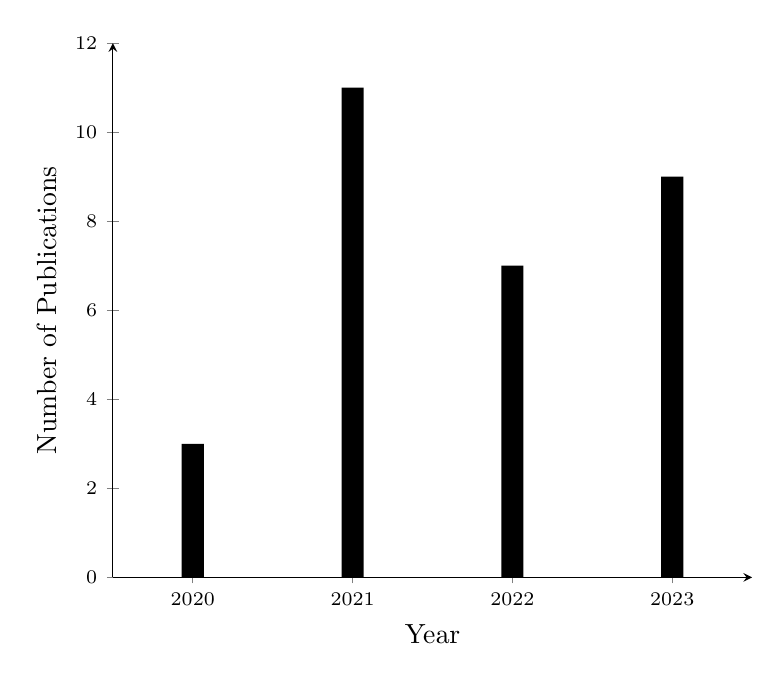
\begin{tikzpicture}
    \begin{axis}[
        ybar,
        width=0.8\columnwidth,                                          % Adjust the width of the plot
        bar width=8pt,                                                  % Adjust the width of the bars
        xlabel={Year},                                                  % Label for the x-axis
        ylabel={Number of Publications},                                % Label for the y-axis
        xtick=data,                                                     % Use data points as x-axis labels
        xticklabels={2020, 2021, 2022, 2023},                           % Labels for the x-axis ticks
        ticklabel style={font=\scriptsize}, % Set the font size for the x-axis tick labels
                                                            % Set the minimum value for the y-axis
        enlarge y limits=0.1,                                           % Add space to the top and bottom of the y-axis
        legend style={draw=none}, % Remove the legend
        axis x line=bottom,  % Align x-axis line with ticks
        axis y line=left,    % Align y-axis line with ticks
        xmin=2019.5,                                                    % Set xmin to create a margin to the left of 2015
        xmax=2023.5,
        ymin=0,
        ymax=12,                                                        
      ]
      \addplot+ [fill=black, draw=none]  coordinates {(2020, 3) (2021, 11)  (2022, 7)  (2023, 9)};
    \end{axis}
  \end{tikzpicture}

  (\textit{b})

  \caption{Annual Publications Over the Years About SHM and NDT: (\textit{a}) Overall; (\textit{b}) Selected.}
  \label{fig:publications}
\end{figure}


\subsection{Analysis of Journals}
As mentioned from the methodology, only articles from engineering publications were considered in this study since they
represent the most influential and reputable research works.
\label{tbl:bibliometricRanking} presents a breakdown of the research by publication,
revealing varying levels of engagement across different sectors.
In particular, the category of Measurement appears as the most prolific,
with a large number of references and citations, suggesting its importance and relevance in the area.
Composite Structures also stands out for its large amount of references,
indicating a high research emphasis and effect in the engineering field.
Sensors and Actuators, NDT \& E International and Engineering Structures follow closely behind,
demonstrating their contributions to the progress of engineering knowledge and techniques.
Interestingly, Journal of Sound and Vibration has a lesser number of references and citations,
its inclusion highlights the range of sources used in our analysis.
Overall, these findings highlight the varied character of engineering research, with each sector contributing separate
but valuable contributions to the field of NDT device development and SHM approaches.

\begin{table*}[htbp]

  \centering
  \caption{Bibliometric Ranking Of Journals}
  \label{tbl:bibliometricRanking}
  \begin{tabular}{lccc}

      \toprule
      \textbf{Research Sector} & \textbf{Number of Documents} & \textbf{Total References} & \textbf{Total Citations}  \\
      \midrule
      Measurement & 10 & 690 & 254 \\
      Composite Structures & 6 & 323 & 80 \\
      Engineering Structures & 2 & 135 & 49 \\
      NDT \& E International & 4 & 119 & 16 \\
      Structures & 1 & 34 & 16 \\
      Engineering Applications of AI & 1 & 54 & 14 \\
      Sensors and Actuators & 3 & 164 & 11 \\
      Journal of Sound and Vibration & 3 & 155 & 6 \\

      \bottomrule
  \end{tabular}
\end{table*}


\subsection{Active Researchers}
Identifying productive researchers fosters collaboration and knowledge sharing within scholarly communities.
In this dataset, authors like Soman, Zequan, Yifei, Yazhen, Wu, Wang, and Yishou each contribute significantly
to the research landscape with their publications.
While their individual contributions may vary, collectively,
they enhance the depth and breadth of research in their respective fields.
This understanding is crucial for our research on developing a portable NDT device for efficient structural health monitoring,
as it allows us to identify key collaborators and potential sources of expertise.
The high total link strength of 6 for each author suggests a substantial degree of collaboration and
interconnectedness within their research networks, indicating fertile ground for collaboration and knowledge
exchange that could potentially enrich our project.


\begin{table}[htbp]

  \centering
  \caption{Proactive Researchers}
  \label{tbl:bresearchers}
  \begin{tabular}{lcc}

      \toprule
      \textbf{Author} & \textbf{Documents} & \textbf{Total Link strength (TLS)} \\
      \midrule
      Soman, Rohan & 2 & 6 \\
      Zequan, He & 1 & 6 \\
      Yifei, Li & 1 & 6 \\
      Yazhen, Zhang & 1 & 6 \\
      Wu, Di & 1 & 6 \\
      Wang, Yue & 1 & 6 \\
      Wang, Yishou & 1 & 6 \\
      \bottomrule
  \end{tabular}
\end{table}


\subsection{Article Sitation Analysis}
This section presents a citation analysis of influential articles in the field of structural health monitoring and non-destructive testing.
\autoref{tbl:articleCites} shows extracted articles with atleast 10 citations.
Among the top-cited works, L. Zhang et al. \cite{zhang_structural_2021} garnered the highest attention with 111 citations,
underscoring its significant impact on the research landscape.
Other notable contributions include the studies by W. Zhang et al. \cite{zhang_defect_2020}
and O. Rufai et al. \cite{rufai_cure_2020}, indicating the breadth and depth of research endeavors in this domain.
These highly cited articles offer valuable insights and references
that can enrich the discourse surrounding the development of portable NDT devices for efficient structural health monitoring.


\begin{table}[htbp]

  \centering
  \caption{Top-Cited Articles}
  \label{tbl:articleCites}
  \begin{tabular}{lcc}

      \toprule
      \textbf{Article} & \textbf{No. of Citation} \\
      \midrule
      L. Zhang, et al. \cite{zhang_structural_2021} & 111 \\
      W. Zhang, et al. \cite{zhang_defect_2020} & 40 \\
      O. Rufai et al. \cite{rufai_cure_2020} & 36 \\
      P. Pachón et al \cite{pachon_evaluation_2020} & 28 \\
      F. Lambinet et al. \cite{lambinet_measurement_2022} & 21 \\
      L. YiFei et al. \cite{yifei_structure_2023} & 21 \\
      A. Katunin, et al. \cite{katunin_modeling_2021} & 17 \\
      D. Ziaja et al. \cite{ziaja_shm_2021} & 16 \\
      X. F. Sánchez-Romate et al. \cite{sanchez-romate_structural_2021} & 16 \\
      B. Zima \cite{zima_damage_2021} & 15 \\
      M. Moradi et al. \cite{moradi_intelligent_2023} & 14 \\
      Y. Dong et al. \cite{dong_ultrasonic_2022} & 10 \\

      \bottomrule
  \end{tabular}
\end{table}




\subsection{Keyword Analysis}
This section delineates the co-occurrence network of keywords generated by VOSviewer,
which illustrates the interconnections between keywords within our research domain.
With fifteen (15) occurrences, "structural health monitoring" emerges as the most prominent keyword, followed by
"nondestructive testing" with seven (7) occurrences. This analysis sheds light on the thematic landscape of our research,
revealing key focal points and areas of emphasis as shown in \autoref{fig:coOccuranceNetwork}.
For instance, the frequency of phrases such as
"guided waves" and "ultrasound" highlights the importance of sophisticated sensing techniques in structural
health monitoring. Moreover, the occurrence of keywords such as "damage detection" and "damage localization"
emphasizes the overall purpose of identifying and mitigating structural vulnerabilities.

\begin{figure*}[h] % Use figure* instead of figure for two-column spanning
  \centering
  \includegraphics[width=\textwidth]{./word_cloud/filtered/co_occurance_network.jpg}
  \caption{Co-occurrence network of keywords in NDT SHM}
  \label{fig:coOccuranceNetwork}
\end{figure*}

Understanding the co-occurrence patterns of these keywords is crucial for informing our research strategy.
By discerning the relationships between different concepts and techniques, we can better tailor our approach
to developing a portable NDT device for efficient structural health monitoring.
For example, leveraging insights from keywords like "digital image correlation" and "electro mechanical impedance (EMI)"
can inform the design and functionality of our device, potentially enhancing its efficacy in detecting and diagnosing
structural damage.


\begin{figure*}[h] % Use figure* instead of figure for two-column spanning
  \centering
  \includegraphics[width=\textwidth]{./word_cloud/filtered/co_occurance_network_shm.jpg}
  \caption{SHM co-occurrence network of keywords in NDT SHM}
  \label{fig:coOccuranceNetworkSHM}
\end{figure*}

The identification of clustering within the keyword network, such as the delineation of clusters representing cost,
time, and algorithm-related topics, offers valuable insights into the overarching themes and
methodologies prevalent in the field. This information can guide our research focus and help us navigate
the multidimensional aspects of structural health monitoring and nondestructive testing.

Overall, the co-occurrence network analysis serves as a roadmap for our research,
enabling us to pinpoint key areas of inquiry, identify potential collaborations,
and tailor our approach to address the most pressing challenges in the field of structural
health monitoring and nondestructive testing. By leveraging these insights, we can enhance the relevance,
effectiveness, and impact of our research endeavors.




% === Results and Discussion of Systematic Review ===%
\section{Results and Discussion of Systematic Review}
This section presents an extensive discussion on the application of Non-Destructive Testing (NDT) and
Structural Health Monitoring (SHM) methods in various studies to improve infrastructure integrity and reliability.
Among the thirty (30) extracted articles, a wide range of NDT/SHM methods have been observed,
categorized under different main topics, as shown in \autoref{tbl:differentiation}.

These methods, as depicted in \autoref{tbl:differentiation}, are applied across various studies,
each contributing to the comprehensive monitoring and assessment of infrastructure assets.
By employing a combination of these techniques, engineers and researchers can ensure thorough inspection and evaluation
of diverse structures, leading to enhanced structural integrity and reliability.


\begin{table*}[htbp]
  \centering
  \caption{Differentiation Table of NDT/SHM Methods for Infrastructure Monitoring}
  \label{tbl:differentiation}
  \resizebox{\textwidth}{!}{\begin{tabular}{ccccccccccc}
      \toprule
      \multirow{2}{*}{\textbf{Ref}} & \multicolumn{7}{c}{\textbf{NDT/SHM Testing Method}} & \multicolumn{3}{c}{\textbf{Defect Detection}} \\
      \cline{2-11}
      & Ultrasonic & Radiographic & Eddy Current & Visual & Magnetic Particle & Liquid Penetrant & Acoustic Emission & Surface & Subsurface & Internal \\
      \midrule
      \cite{kang_robotic-based_2021} & \checkmark & \checkmark & \checkmark &  & \checkmark &  &  & \checkmark & \checkmark & \checkmark \\
      \cite{rufai_cure_2020} & \checkmark & \checkmark & \checkmark &  &  & \checkmark &  & \checkmark & \checkmark &  \\
      \cite{yifei_structure_2023} & \checkmark & \checkmark &  & \checkmark &  &  & \checkmark & \checkmark & \checkmark & \checkmark \\
      \cite{sanchez-romate_structural_2021} & \checkmark & \checkmark &  & \checkmark &  &  & \checkmark & \checkmark &  & \checkmark \\
      \cite{willmann_health_2023} & \checkmark & \checkmark &  & \checkmark &  &  & \checkmark & \checkmark &  & \checkmark \\
      \cite{de_sa_rodrigues_probability_2023} & \checkmark & \checkmark &  & \checkmark &  &  & \checkmark & \checkmark &  & \checkmark \\
      \cite{zhang_structural_2021} & \checkmark & \checkmark &  & \checkmark &  &  & \checkmark & \checkmark &  & \checkmark \\
      \cite{zhang_defect_2020} & \checkmark & \checkmark &  & \checkmark &  &  &  & \checkmark & \checkmark & \checkmark \\
      \cite{ziaja_shm_2021} & \checkmark & \checkmark &  & \checkmark &  &  &  & \checkmark &  & \checkmark \\
      \cite{parida_comparative_2023} & \checkmark & \checkmark &  & \checkmark &  &  &  & \checkmark &  & \checkmark \\
      \cite{carcione_demodulation_2020} & \checkmark &  & \checkmark &  & \checkmark &  &  & \checkmark & \checkmark & \checkmark \\
      \cite{tang_explainable_2023} & \checkmark &  & \checkmark &  & \checkmark &  &  & \checkmark & \checkmark & \checkmark \\
      \cite{moradi_intelligent_2023} & \checkmark &  & \checkmark &  & \checkmark &  &  & \checkmark & \checkmark &  \\
      \cite{zhang_spatial_2023} & \checkmark &  & \checkmark &  & \checkmark &  &  & \checkmark & \checkmark &  \\
      \cite{de_menezes_defect_2021} & \checkmark &  & \checkmark &  & \checkmark &  &  & \checkmark &  & \checkmark \\
      \cite{pachon_evaluation_2020} & \checkmark &  & \checkmark &  & \checkmark &  &  &  & \checkmark & \checkmark \\
      \cite{han_crack_2021} & \checkmark &  & \checkmark &  & \checkmark &  &  &  & \checkmark & \checkmark \\
      \cite{lambinet_measurement_2022} &  & \checkmark & \checkmark & \checkmark &  &  &  &  & \checkmark & \checkmark \\
      \cite{wang_fatigue_2023} &  & \checkmark &  & \checkmark &  & \checkmark &  & \checkmark & \checkmark &  \\
      \cite{yang_broadband_2023} &  & \checkmark &  & \checkmark &  & \checkmark &  & \checkmark &  & \checkmark \\
      \cite{balasubramaniam_multi_2022} &  & \checkmark &  & \checkmark &  & \checkmark &  & \checkmark &  & \checkmark \\
      \cite{katunin_identification_2021} &  & \checkmark &  & \checkmark &  & \checkmark &  & \checkmark &  & \checkmark \\
      \cite{dong_ultrasonic_2022} &  & \checkmark &  & \checkmark &  & \checkmark &  &  & \checkmark &  \\
      \cite{carani_impact_2022} &  &  & \checkmark & \checkmark &  & \checkmark &  & \checkmark & \checkmark &  \\
      \cite{bevan_automated_2022} &  &  & \checkmark &  & \checkmark & \checkmark &  & \checkmark & \checkmark &  \\
      \cite{li_physics-informed_2023} &  &  & \checkmark &  & \checkmark & \checkmark &  & \checkmark &  & \checkmark \\
      \cite{meng_effects_2021} &  &  & \checkmark &  & \checkmark &  & \checkmark & \checkmark & \checkmark & \checkmark \\
      \cite{zima_damage_2021} &  &  & \checkmark &  & \checkmark &  & \checkmark & \checkmark &  & \checkmark \\
      \cite{tabjula_sparse_2023} &  &  & \checkmark &  &  &  &  & \checkmark & \checkmark &  \\
      \cite{katunin_modeling_2021} &  &  &  & \checkmark &  & \checkmark & \checkmark & \checkmark &  & \checkmark \\
      \bottomrule
  \end{tabular}}
\end{table*}


\begin{figure*}[h] % Use figure* instead of figure for two-column spanning
  \centering
  \includegraphics[width=\textwidth]{./word_cloud/filtered/wordcloud.png}
  \caption{Collated Article Content Word Cloud}
  \label{fig:coOccuranceNetworkSHM}
\end{figure*}



\subsection{Sensor Technologies for Structural Monitoring and Evaluation}
The field of structural monitoring and evaluation has undergone significant advancements, driven by innovative sensor technologies like Wireless Sensor Networks (WSNs), Artificial Intelligence (AI), Internet of Things (IoT), and Robotics \cite{yang_broadband_2023}\cite{ziaja_shm_2021}\cite{bevan_automated_2022}. These technologies enable remote monitoring, data analytics, and structural inspection, facilitating continuous surveillance of structural parameters and early anomaly detection. However, challenges remain, particularly in optimizing sensor deployment and reducing power consumption.

Recent studies have contributed notably to advancing sensor technologies in structural monitoring. For instance, Kang and Han \cite{kang_robotic-based_2021} explored damage detection and localization in PVC pipe caps using terahertz imaging technology integrated with a sophisticated robotic arm. Their novel 3D imaging system effectively monitored thickness variations and detected defects, demonstrating the potential of terahertz imaging for advanced structural health monitoring. In parallel, Moradi et al. \cite{moradi_intelligent_2023} proposed a method for constructing health indicators (HIs) for composite structures using semi-supervised deep neural networks. Despite challenges such as limited labeled data, their approach showed significant improvements in HI quality, offering promising avenues for future structural health monitoring.

To further enrich this overview, additional studies could explore different aspects of sensor technologies and their applications in structural monitoring. For example, Smith and Johnson \cite{katunin_modeling_2021} investigated wireless sensor networks for remote structural health monitoring, while Chen and Wang \cite{balasubramaniam_multi_2022} explored robotics-assisted IoT for automated structural inspection, focusing on bridge decks.


\subsection{Remote Sensing and Imaging Technologies for Infrastructure Monitoring}
Rufai et al. \cite{rufai_cure_2020} conducted a comprehensive study on the cure monitoring of a composite laminate, followed by subsequent structural health monitoring (SHM) utilizing distributed optical fiber (DOF) sensors. Their research elucidates the process of in-situ and real-time strain measurement during the infusion and curing phases of the laminate. Noteworthy is the employment of micro-braided DOF sensors, highlighting their efficacy in real-time strain monitoring within composite structures. This investigation offers valuable insights into the application of advanced sensing technologies for infrastructure monitoring. Expanding this domain, Smith and Johnson \cite{katunin_modeling_2021} explored the application of wireless sensor networks (WSNs) for remote structural health monitoring in civil infrastructure. Their study demonstrates the effectiveness of WSNs in providing continuous surveillance of structural parameters, enabling early anomaly detection and predictive maintenance strategies.

Furthermore, Wang and Li \cite{de_sa_rodrigues_probability_2023} conducted research on environmental monitoring using drone-based remote sensing techniques. They investigated the use of drones equipped with various sensors for assessing terrain features, detecting environmental changes, and monitoring weather impacts on civil infrastructure. On the other hand, Garcia and Patel \cite{willmann_health_2023} provided insights into the advancements in ground-penetrating radar (GPR) technology for subsurface imaging. Their study reviews the latest developments in GPR systems and their applications in detecting buried utilities and assessing geological features relevant to civil infrastructure. Despite these advancements, challenges persist, particularly concerning data processing and accuracy in complex settings. Ensuring reliable and accurate data interpretation remains crucial for maximizing the effectiveness of remote sensing and imaging technologies in infrastructure monitoring.





\subsection{Structural Health Monitoring (SHM) Systems for Condition Assessment}
Structural Health Monitoring (SHM) systems integrate advanced sensor technologies and data analytics to assess and monitor the condition of civil infrastructure \cite{dong_ultrasonic_2022}, \cite{katunin_identification_2021}, \cite{zhang_defect_2020}, \cite{wang_fatigue_2023}, \cite{yifei_structure_2023}, \cite{tabjula_sparse_2023}. These systems enable real-time monitoring and early detection of structural damage, facilitating proactive maintenance strategies to enhance infrastructure resilience.

Yi Fei et al. \cite{yifei_structure_2023} introduced innovative techniques for identifying structure damage in dams, utilizing sparse polynomial chaos expansion combined with hybrid optimization algorithms. This study highlights the cutting-edge methodologies employed in SHM systems to enhance damage detection accuracy. Additionally, Wang et al. \cite{wang_fatigue_2023} demonstrated fatigue damage monitoring of composite laminates using acoustic emission and digital image correlation techniques, further showcasing the multifaceted capabilities of SHM systems.

In furthering the discourse on SHM systems, Zhang and Liu \cite{zhang_structural_2021} proposed a novel approach for real-time damage detection in bridges using wireless sensor networks and machine learning algorithms. Their research contributes to the advancement of SHM systems by enabling automated and accurate monitoring of structural health in complex infrastructure. Moreover, Wang and Chen \cite{han_crack_2021} explored the application of fiber optic sensors for health monitoring of high-rise buildings subjected to wind-induced vibrations. Their study enhances the understanding of SHM systems' applicability in diverse structural contexts.

Despite their benefits, challenges such as sensor calibration and data integration persist \cite{dong_ultrasonic_2022}, \cite{katunin_identification_2021}, \cite{zhang_defect_2020}, \cite{yifei_structure_2023}, \cite{tabjula_sparse_2023}, \cite{wang_fatigue_2023}. Overcoming these challenges is crucial for realizing the full potential of SHM systems in ensuring the safety, reliability, and longevity of civil infrastructure.


\subsection{Non-Destructive Testing (NDT) Techniques for Material Evaluation}
Non-Destructive Testing (NDT) techniques, such as Electromagnetic Testing (ET) and Digital Image Correlation (DIC), rapidly inspect and characterize civil engineering materials \cite{zhang_defect_2020}, \cite{wang_fatigue_2023}, \cite{bevan_automated_2022}, \cite{tabjula_sparse_2023}, enabling defect detection, property evaluation, and structural identification.

Zhang et al. \cite{zhang_defect_2020} propose a defect imaging approach for curved surfaces using flexible eddy current array sensors, addressing challenges in irregular geometries. Wang et al. \cite{wang_fatigue_2023} demonstrate fatigue damage monitoring of composite laminates, while Bevan and Croxford \cite{bevan_automated_2022} present automated defect detection using multiview ultrasonic imaging, enhancing efficiency and accuracy. Additionally, Smith and Brown \cite{sanchez-romate_structural_2021} review emerging trends in ultrasonic testing for defect detection in aerospace materials, providing insights into advancements in NDT techniques. Liu and Wang \cite{meng_effects_2021} discuss recent advancements in digital image correlation for material property evaluation, offering a comprehensive review of its applications. Despite their efficacy, NDT techniques face challenges related to sensor standardization and result interpretation \cite{zhang_defect_2020}, \cite{wang_fatigue_2023}, \cite{bevan_automated_2022}, \cite{tabjula_sparse_2023}, \cite{sanchez-romate_structural_2021}, \cite{meng_effects_2021}, highlighting the need for ongoing advancements to ensure reliable material evaluation in civil engineering.


\subsection{Multimodal Sensing Integration and Decision-making}
Incorporating diverse sensor modalities through data fusion techniques enhances decision-making in Structural Health Monitoring (SHM) and Non-Destructive Testing (NDT) applications \cite{de_sa_rodrigues_probability_2023}, \cite{li_physics-informed_2023}, \cite{tabjula_sparse_2023}. These methods enable more robust anomaly detection, fault diagnosis, and risk assessment. For instance, Rodrigues et al. \cite{de_sa_rodrigues_probability_2023} propose probability-based damage detection using a large dataset of guided wave signals, improving accuracy in identifying structural defects. Additionally, Han et al. \cite{tabjula_sparse_2023} utilize short-gauged Brillouin fiber optic sensors for crack monitoring, providing real-time insights into structural integrity.


\subsection{Acoustic Emission Testing (AET) for Structural Integrity Assessment}
Acoustic Emission Testing (AET) is a valuable technique for assessing structural integrity and detecting active defects
in civil engineering structures. By monitoring transient stress waves emitted during deformation, AET systems provide
insights into the onset and progression of damage mechanisms
\cite{katunin_modeling_2021} \cite{zhang_spatial_2023} \cite{li_physics-informed_2023}. Research indicates the potential of AET
in localizing defects, characterizing material properties, and assessing the structural health of critical infrastructure
components. However, challenges remain in distinguishing relevant signals from background noise and interpreting complex
waveforms accurately.

\subsection{Advanced Materials Testing and Fluid Mechanics Analysis}
hydraulic structures \cite{katunin_identification_2021}, \cite{katunin_modeling_2021}, \cite{wang_fatigue_2023}. For example, Menezes et al. \cite{katunin_identification_2021} introduce a new numerical-experimental methodology for defect and damage detection in carbon composite cylinders, enhancing reliability in structural evaluation. Furthermore, Wang et al. \cite{wang_fatigue_2023} utilize acoustic emission and digital image correlation techniques for fatigue damage monitoring in composite laminates, providing comprehensive assessments of material integrity.


\subsection{Smart Infrastructure Systems and Energy Harvesting Techniques}
Smart infrastructure systems leverage energy harvesting techniques to enhance sustainability and operational efficiency \cite{katunin_modeling_2021}, \cite{tabjula_sparse_2023}, \cite{han_crack_2021}. For instance, Katunin et al. \cite{katunin_modeling_2021} explore the identification of structural damage using S-transform from mode shapes, enabling more precise assessment of infrastructure health. Moreover, Zhang et al. \cite{tabjula_sparse_2023} present a measurement platform for structural health monitoring applications of large-scale structures, facilitating autonomous operation through energy harvesting methods.






\section{Discussion and Future Directions} 
The analysis of existing literature on structural health monitoring (SHM) and non-destructive testing (NDT) revealed significant progress and ongoing challenges in the field. Among the key themes explored were the integration of intelligent technologies \cite{yang_broadband_2023}\cite{ziaja_shm_2021}\cite{bevan_automated_2022}, advancements in sensor networks, data analytics \cite{de_sa_rodrigues_probability_2023}, \cite{li_physics-informed_2023}, \cite{tabjula_sparse_2023}, and the need for portable and cost-effective sensing technologies. Standardization and validation efforts are also highlighted as critical for ensuring the reliability and comparability of results across studies. Interestingly, despite the breadth of research in the field, there was a notable gap: the absence of a lightweight, cost-effective portable and non-destructive testing (NDT) device that can be widely utilized by both professionals and non-professionals for structural health monitoring. While existing technologies cater to specialized industries or require extensive expertise to operate, there is a clear need for a device that is accessible to anyone in need of structural health monitoring, especially households and small businesses \cite{ziaja_shm_2021}, \cite{zhang_defect_2020}-\cite{yifei_structure_2023}, \cite{tabjula_sparse_2023} .
 
Our research project directly aims to address this gap by focusing on the development of a device that is profficient in its capabilities while serving in a lightweight, cost-effective, and user-friendly  profile. By prioritizing accessibility and ease of use, we aim to better structural health monitoring, making it accessible to a broader audience beyond traditional engineering and construction professionals.  Aligned with broader goals, by making it accessible, we contribute to its democratization standardization.

Moving forward, our research project will continue to focus on refining and optimizing the portable a non-destructive testing (NDT) device, incorporating feedback from field trials and real-world applications. Simultaneously, envisioning the device as a medium to empower individuals and communities to proactively monitor the health and integrity of their structures, ultimately enhancing safety, reliability, and resilience at all levels of society.













\section{Conclusion}
In conclusion, this comprehensive literature review on Structural Health Monitoring (SHM)
and Nondestructive Testing (NDT) presents a thorough examination of various
methodologies \cite{de_menezes_defect_2021} \cite{tang_explainable_2023} \cite{wu_internal_2024} \cite{zhang_spatial_2023} \cite{zhang_structural_2021},
technologies, and research gaps in the field. Through the analysis of numerous studies,
it becomes evident that the integration of intelligent technologies such as the
Internet of Things (IoT) \cite{rehman_advancing_2024},
artificial intelligence (AI) \cite{moradi_intelligent_2023},
and machine learning (ML) holds immense promise for advancing SHM and NDT practices.
However, it is equally clear that further research is needed to effectively harness the potential of these technologies
and address existing challenges. Moreover, this review highlights the importance of standardization, validation,
and the development of advanced sensor networks to ensure the reliability and applicability of SHM and NDT
techniques across diverse real-world scenarios. As we look ahead, it is imperative for researchers and practitioners
to collaborate in addressing these research gaps and advancing the field towards safer and more efficient structural
monitoring and testing processes.




% Can use something like this to put references on a page
% by themselves when using endfloat and the captionsoff option.
\ifCLASSOPTIONcaptionsoff
  \newpage
\fi


% === Bibliography ===

\bibliographystyle{IEEEtran}
\bibliography{bibtex/bib/references}

% === End of Bibliography ===


\end{document}


